\documentclass[a4paper,12pt]{book}
\usepackage[utf8]{inputenc}
\usepackage{graphicx}
\usepackage{hyperref}
\usepackage{longtable}

\begin{document}

\author{Christopher Wells}
\title{A Code-Oriented Guide to Clustering and Classification in R}
\date{\today}

\frontmatter
\maketitle

Available under the \href{https://creativecommons.org/licenses/by-sa/4.0/}{CC BY-SA 4.0} license, feel free to modify and redistribute this document under the terms of the license.
\tableofcontents

\mainmatter
\chapter{General Information}

\section{Reading in data files}
When you are trying to cluster and classify data, typically the first step is reading in the data from a file. There are several different ways that data is typically stored in a data file, the most common formats are comma separated values (csv) or tab separated values (tsv). For both of these types of files, R has some inbuilt functions for reading them into data frames.

Typically csv files tend to be easier to read in, as they usually have proper column labels and very simple value separation. Tsv files can vary in their formatting between tabs and different types of spacing, and often do not have column labels.

\subsection{CSV files}
Csv files are very easy to read in with R. Let's consider the following csv file.

\begin{verbatim}
id,mag,amp,error
00001,20.123,19.312,0.2486362
00003,19.02,20.2,0.47823
00004,18.8,21.389,0.277669
\end{verbatim}

In R you can read in csv files using the \verb|read.csv| function. We must note that this csv file has column headers, so we need to add an argument to indicate this.

\begin{verbatim}
myData <- read.csv("data.csv", header=TRUE)
\end{verbatim}

\subsection{TSV files}
Let's take a look at a more unusual tsv file and read it in to R. This tsv file uses a special format that allocates a specific width to each column, such that a non-standard amount of additional spaces are added for padding.

\begin{verbatim}
00001  20.123 19.312  0.2486362
00003  19.023 20.213  0.4782373
00004  18.789 21.389  0.2776688
\end{verbatim}

To read this data in with R we need to use the \verb|read.table| function. We must note that the data file does not have column headers, and does not have a sepcific separater string.

\begin{verbatim}
myData <- read.table("data.tsv")
\end{verbatim}

The resulting data frame will include all of the given data, however its column names with be generic. The next thing we will need to do is to label the columns. In R there are many different ways to rename columns, however since we want to rename all of the columns we can make use of the \verb|names| function.

\begin{verbatim}
names(myData) <- c("id", "mag", "amp", "error")
\end{verbatim}

\section{Normalizing data}
Before you do any sort of clustering on data, you should first normalize the data. Datasets generally have features that are of different units and ranges of values and this must be taken into account when performing clustering.

To normalize a data frame in R, you can use the \verb|scale| function.

\begin{verbatim}
normalizedData <- scale(myData)
\end{verbatim}

\section{Misc. Functions}

\subsection{Conversion functions}
To convert a numerical factor into the corresponding num representations you can use a combination of the \verb|as.character| and \verb|as.numeric| functions. Any values that are not able to be converted into numeric values will be converted into \verb|NA|s.

\begin{verbatim}
myData$phi31 <- as.numeric(as.character(myData$phi31))
\end{verbatim}

\subsection{Mapping functions}
To map a function over the rows of a data frame and be able to access specific columns you can use the \verb|with| function.

\begin{verbatim}
myData$logMag <- with(myData, log(mag))
\end{verbatim}
\chapter{Clustering}

\section{Kmeans}
Kmeans is a good general clustering technique. It attempts to group your data into a specified number of clusters. Luckily R has an inbuilt  function ``kmeans'' that can be used.

\begin{center}
	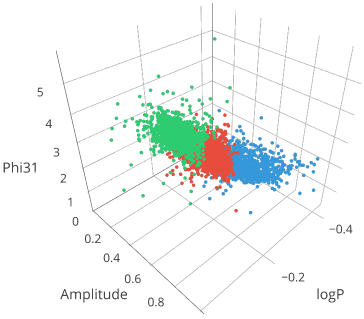
\includegraphics[width=0.5\textwidth]{images/kmeans_01.png}
\end{center}

To use kmeans you must first pull out the features of the data that you want to cluster on. Then you can pass the data into the kmeans function, specifying the number of clusters that you want, and it will return information about the generated clusters.

\begin{verbatim}
myData <- offABClustering[,c("logP", "phi31", "amp.I")]
clusters <- kmeans(myData, 3)
\end{verbatim}

If you want to pull out just the cluster ids that kmeans generates in order to store that information in your dataframe, you can pull it out as a ``cluster'' feature and turn it into a factor.

\begin{verbatim}
offABClustering$cluster <- factor(clusters$cluster)
\end{verbatim}

\section{Support Vector Machines}
Support Vector Machines are a clustering technique that tries to separate data using a linear line, however through the use of kernels it is able transform the data space to give clusters that are non-linear in normal space.

\begin{center}
	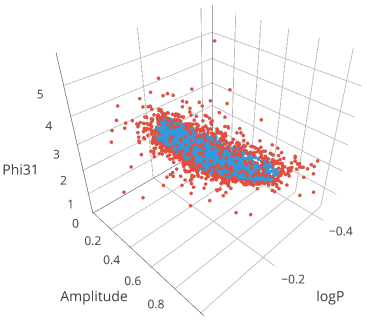
\includegraphics[width=0.5\textwidth]{images/ksvm_01.png}
\end{center}

There are several libraries in R for using support vector machines (SVM).

\begin{itemize}
	\item kernlab
	\item e1071
\end{itemize}

Let's take a look at the kernlab library for now. To cluster data using an SVM with kernlab you need to pull out just the features you want and then convert that dataframe into a matrix. Then you can pass the resulting matrix into the ksvm function.

\begin{verbatim}
myData <- offABClustering[,c("logP", "phi31", "amp.I")]
myMatrix <- as.matrix(myData)
ksvmModel <- ksvm(myMatrix)
\end{verbatim}

The ksvm function will give you a model which you can then use to classify your data into the calculated clusters.

\begin{verbatim}
predictions <- predict(ksvmModel, myData)
offABClustering$cluster <- as.factor(predictions)
\end{verbatim}

\subsection{Kernels}
The ksvm function offers a few different kernels that you can use to change how it clusters the data. Each of these kernels will cluster the data into different ``shapes'' ranging from linear separations to rings. It looks like ksvm uses the ``rbfdot'' kernel by default.

\begin{itemize}
	\item rbfdot Radial Basis kernel "Gaussian"
	\item polydot Polynomial kernel
	\item vanilladot Linear kernel
	\item tanhdot Hyperbolic tangent kernel
	\item laplacedot Laplacian kernel
	\item besseldot Bessel kernel
	\item anovadot ANOVA RBF kernel
	\item splinedot Spline kernel
\end{itemize}

You can specify the kernel to be used in ksvm, by adding a kernel parameter where you pass in the name of the kernel you want to use as a string.

\begin{verbatim}
ksvmModel <- ksvm(myMatrix, kernel = "vanilladot")
\end{verbatim}

\begin{longtable}{ c c }
	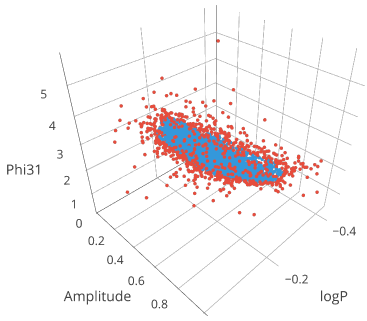
\includegraphics[width=0.3\paperwidth]{images/ksvm_rbfdot.png} & 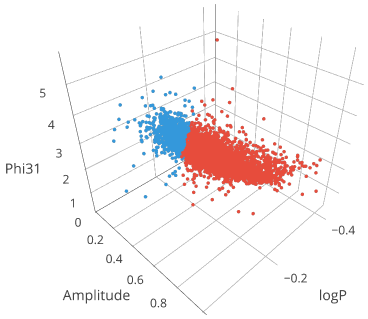
\includegraphics[width=0.3\paperwidth]{images/ksvm_polydot.png} \\
	rbfdot & polydot \\
	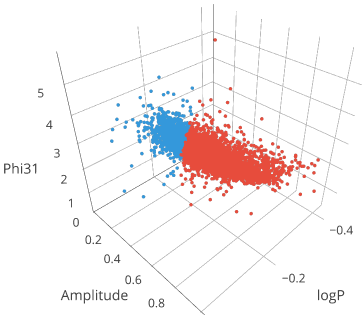
\includegraphics[width=0.3\paperwidth]{images/ksvm_vanilladot.png} & 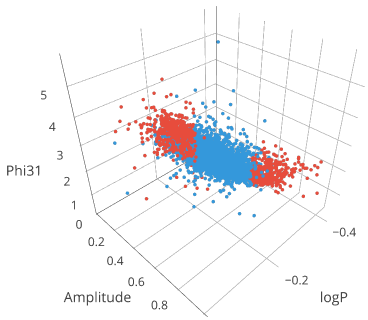
\includegraphics[width=0.3\paperwidth]{images/ksvm_tanhdot.png} \\
	vanilladot & tanhdot \\
	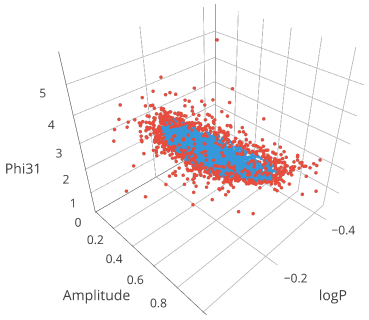
\includegraphics[width=0.3\paperwidth]{images/ksvm_laplacedot.png} & 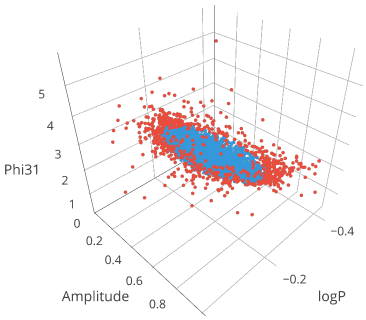
\includegraphics[width=0.3\paperwidth]{images/ksvm_besseldot.png} \\
	laplacedot & besseldot \\
	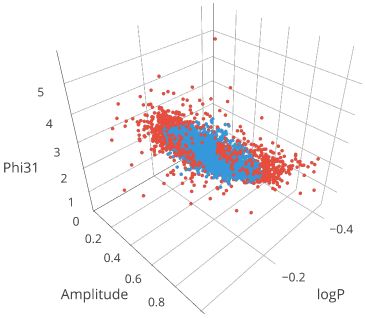
\includegraphics[width=0.3\paperwidth]{images/ksvm_anovadot.png} & 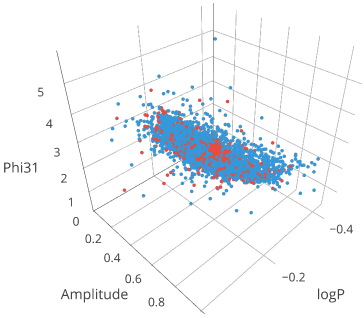
\includegraphics[width=0.3\paperwidth]{images/ksvm_splinedot.png} \\
	anovadot & splinedot \\
\end{longtable}



\backmatter
% bibliography, glossary and index would go here.

\end{document}